\chapter{Analysis of Carbon Tariffs impacts}
\label{sec:theorethical}

\section{Theoretical Model}

In a series of counterfactual analyses, \textcite{Larch2017} study the consequences of introducing carbon tariffs on trade flows, welfare, and carbon emissions, by decomposing the changes in emissions into three effects: scale, composition, and technique. To do~so, they take advantage of a gravity model, which is a workhorse framework employed in the field of international trade. The power of this tool lies in the gravity equation, which can describe the link between trade flows and the size, distance, and border resistance~of~countries.

Firstly, they introduce the presence of more sectors: a non-tradable sector $S$ and $L$ tradable ones ($l$) in all $N$ countries. This enables the detection of how sectors with different carbon intensities respond and interact with each other when a carbon tariff is levied. The utility the representative consumer from country $j$ gains when consuming in sector $l$ is shown in Equation \ref{eq:CESutility} (a):
\begin{flalign}\label{eq:CESutility}
&\scalemath{0.92}{
(a)\;U_l^j= \left[\sum_{i=1}^{N}(\beta_l^i)^{\frac{1-\sigma_l}{\sigma_l}}(q_l^{ij})^{\frac{\sigma_l-1}{\sigma_l}} \right]^{\frac{\sigma_l}{\sigma_l-1}}
\quad(b)\;U^j=(U_S^j)^{\gamma_S^j}\left[\prod_{l\in\mathcal{L}}(U_l^j)^{\gamma_l^j}\right]\left[\frac{1}{1+(\frac{1}{\mu^j}\sum_{i=1}^{N}E^i)^2}\right]}&
\end{flalign}
where $\sigma_l$ is the elasticity of substitution of sector $l$, $\beta_l^i$ is a sector and country-specific distribution parameter, and $q_l^{ij}$ is the quantity of goods from tradable sector $l$ and imported from country $i$ that the representative consumer $j$ consumes. Additionally, Equation \ref{eq:CESutility} (b) measure the total utility of the country's representative consumer $j$ that comes from both types of sectors, $S$ and $L$, discounted for the disutility arising from global carbon emissions. The $\gamma^j$ are elasticities and sum up to $1$, $E^i$ are the emissions produced by country $i$, and $\mu^j$ is the Social Cost of Carbon (SCC) for the affected country $j$, denoting the economic damage caused by an additional unit of emissions.

To afford consumption, the representative consumer in country $j$ earns income $Y^j$ from selling energy, providing labor, and a number of other factors $\mathcal{F}$. Furthermore, the revenues from carbon tariffs imposed on imports from country $i$, i.e. $\sum_{l\in\mathcal{L}}\sum_{i=1}^N(\tau_l^{ij}-1)X_l^{ij}$, are redistributed to the consumer and also feed its income equation. Let's assume that all income in each country is spent, so-called balanced trade assumption, i.e. $Y^j=\mathfrak{X}^j=\mathfrak{X}_S^j+\sum_{l\in\mathcal{L}}\mathfrak{X}_l^j$, we can now find the demand of country $j$ for goods from country $i$ in sector $l$, as in Equation \ref{eq:demandPrice} (a):
\begin{flalign}\label{eq:demandPrice}
&(a)\;q_l^{ij}=\left(\frac{\beta_l^ip_l^{ij}}{P_l^j}\right)^{-\sigma}\left(\frac{\beta_l^i\mathfrak{X}_l^j}{P_l^j}\right)\quad(b)\;P_l^j=\left[\sum_{i=1}^N(\beta_l^ip_l^{ij})^{1-\sigma_l}\right]^{\frac{1}{1-\sigma_l}}&
\end{flalign}
where $\mathfrak{X}_l^j$ is the total expenditure of country $j$ in sector $l$, $p_l^{ij}$ is the price in country $j$ for goods from sector $l$ coming from country $i$. Instead, $P_l^j$ is the sectoral price index, giving an overall measure for the prices in sector $l$. Therefore, from Equation \ref{eq:demandPrice} (a) we can see, for instance, that demand $q_l^{ij}$ increases either if $\mathfrak{X}_l^j$ increases (e.g. thanks to an increase in country income $Y^j$) or if goods from $i$ are more competitive and cheaper relative to the overall price index $P_l^j$ (i.e. a lower $\frac{p_l^{ij}}{P_l^j}$).

Now that we have an endogenous demand function for goods, let's define trade flows.
\begin{flalign}\label{eq:gravity}
&\scalemath{1}{\; X_l^{ij}=\underbrace{\frac{Y_l^i\gamma_l^jY^j}{Y^W}\vphantom{\left(\frac{T_l^{ij}}{\prod_l^iP_l^j}\right)^{1-\sigma}}}_\text{(1)}\underbrace{\left(\frac{T_l^{ij}}{\prod_l^iP_l^j}\right)^{1-\sigma}}_\text{(2)}\underbrace{(\tau_l^{ij})^{-\sigma_l}\vphantom{\left(\frac{T_l^{ij}}{\prod_l^iP_l^j}\right)^{1-\sigma}}}_\text{(3)}}&
%&\scalemath{0.9}{(b)\; \prod_l^i=\left[\sum_{j=1}^N\left(\frac{T_l^{ij}}{P_l^j}\right)^{1-\sigma_l}(\tau_l^{ij})^{-\sigma_l}\gamma_l^j\theta^j\right]^{\frac{1}{1-\sigma_l}}\quad
%(c)\; P_l^j=\left[\sum_{i=1}^N\left(\frac{T_l^{ij}\tau_l^{ij}}{\prod_l^i}\right)^{1-\sigma_l}\theta_l^i\right]^{\frac{1}{1-\sigma_l}}}
\end{flalign}
Equation \ref{eq:gravity} is the extended gravity equation. The trade flows in sector $l$ from country $i$ to $j$ depend: (1) on the relative size of sector $l$ in both countries, the larger the production in this sector and the more is traded; (2) given transport costs $T_l^{ij}$ between the two countries, more is exchanged if the two multilateral resistance terms (i.e. $\prod_l^i$ outward, $P_l^i$ inward) are smaller; (3) larger carbon tariffs $\tau_l^{ij}$ for products coming from $i$ reduce imports. In particular, the two multilateral resistance terms, calculated by taking each pair of countries, play a crucial role in explaining how conditions in all other countries interact with trade between $i$ and $j$.

%Another main contribution of \textcite{Larch2017} is the addition of energy as a production input, yielding a multi-factor Cobb-Douglas production function and, for instance, for sector $l$ this results in $q_l^i=A_l^i(E_l^i)^{\alpha_{lE}^i}\prod_{f\in\mathcal{F}}(V_{lf}^i)^{\alpha_{lf}^i}$. Where $A_l^i$ is a productivity parameter, $E_l^i$ is the energy employed by sector $l$ in country $i$, $V_{lf}^i$ the other factors, $\alpha_{lE}^i$ and $\alpha_{lf}^i$ the cost share for energy and other factors, respectively. As a result, the carbon emissions produced are treated as a byproduct and can be measured in proportion to the energy used.

After welfare (Equation \ref{eq:CESutility} (b)), income, and trade flows (Equation \ref{eq:gravity}), the last key variable investigated is carbon emissions produced. The authors start shaping total emissions for each country as $E^i=(\alpha_{SE}^iY_S^i+\sum_{l\in\mathcal{L}}\alpha_{lE}^iY^i)/e^i$, where $\alpha_{lE}^i$ and $\alpha_{SE}^i$ are the energy cost shares for each sector, and $e^i$ the enegy price in country $i$. Intuitively, the authors treat emissions as a byproduct of the energy used, and the numerator suggests that if energy costs are a significant component of the production costs, production is more energy and carbon-intensive. After some transformations, we can rewrite the total emissions for country $i$  as in Equation \ref{eq:emissions} (a):

\begin{flalign}\label{eq:emissions}
&\scalemath{0.86}{(a)\;E^i=\bar{\alpha}^i_E\frac{\tilde{Y}^i}{P^i}\left(\frac{e^i}{P^i}\right)^{-1}\quad
(b)\;dE^i=\underbrace{\frac{\delta E^i}{\delta(\tilde{Y}^i/P^i)}d(\tilde{Y}^i/P^i)}_\text{(1) scale effect}+\underbrace{\frac{\delta E^i}{\delta \bar{a}^i_E}d\bar{a}^i_E}_\text{(2) composition effect}+\underbrace{\frac{\delta E^i}{\delta (e^i/P^i)}d(e^i/P^i)}_\text{(3) technique effect}}&
\end{flalign}
here, emissions are expressed in real value terms of production and energy prices, while the weighting factor $\bar{\alpha}^i_E$ reflects the average energy costs share. Therefore, total emissions $E^i$ in country $i$ can increase if the real value of overall production increases, but also when production sectoral shares change. The various effects resulting from changes to the variables of the model can be decomposed by taking the total derivative of Equation \ref{eq:emissions} (a), as shown in Equation \ref{eq:emissions} (b).
\begin{flalign}\label{eq:emissionsEffects}
&\scalemath{0.98}{(1)\;\frac{\delta E^i}{\delta(\tilde{Y}^i/P^i)}=\frac{\bar{a}^i_E}{e^i/P^i}>0\quad
(2)\;\frac{\delta E^i}{\delta \bar{a}^i_E}=\frac{\tilde{Y}^i}{e^i}>0\quad
(3)\;\frac{\delta E^i}{\delta (e^i/P^i)}=-\frac{\bar{\alpha^i_E}\tilde{Y}^i/P^i}{(e^i/P^i)^2}<0}&
\end{flalign}
Equation \ref{eq:emissionsEffects} represents a key contribution of \textcite{Larch2017} and describes how total emissions behave when certain variables in the model change, for example, as a result of the introduction of carbon tariffs. In Equation \ref{eq:emissionsEffects},  (1) represents the "scale effect" and indicates that an increase in real value production increases emissions, (2) is the "composition effect" and reflects the sectoral composition of production and its carbon intensity, for example, a carbon-intensive sector increasing its share will result in an increase in total emissions, (3) illustrates the "technique effect", where an increase in real energy prices leads to a decrease in emissions, because higher energy costs encourage producers either to use energy more efficiently or to switch to less energy-intensive (and therefore less carbon-intensive) sectors.

\section{Empirical Strategy}

The analysis of \textcite{Larch2017} compares a benchmark and a counterfactual case without and with carbon tariffs, respectively. To achieve this, they utilize several data sources, outlined in Section \ref{sec:data}, from which they extract or calculate data such as for the benchmark production levels ($Y_b^i$) or the energy cost shares ($\alpha_{lE}^i$). However, there isn't a unique and overarching measure for trade costs $T_l^{ij}$, thus they must be approximated as a function of observable factors and estimated using the gravity equation, Equation \ref{eq:gravity}.

First, the authors approximate $T_l^{ij}$ giving it the form of an exponential function of $K$ observable variables, which results in $T_l^{ij}=\text{exp}\left(\left(\boldsymbol{z}_l^{ij}\right)^\prime\boldsymbol{b}_l\right)$. The $K$ variables they employ are (1) distance, (2) contiguity, whether they have (3) bilateral Regional Trade Agreements (RTA), (4) a common language, (5) a direct colonial link or (6) a common colonizer in the past. Once this formulation for $T_l^{ij}$ is plugged into the gravity equation and after some transformations, Equation \ref{eq:estimate} is used to estimate the coefficients of the factors influencing trade costs:
\begin{flalign}\label{eq:estimate}
&\scalemath{1}{\;X_l^{ij}=\frac{1}{Y^W}\text{exp}\left(\left(\boldsymbol{z}_l^{ij}\right)^\prime\boldsymbol{\beta}_l\right)\left(\tau_l^{ij}\right)^{-\sigma}n_l^im_l^ju_l^{ij}
}&
\end{flalign}
where trade flows $X_l^{ij}$ is the dependent variable, $\boldsymbol{z}_l^{ij}$ is the vector of the mentioned independent variables for each pair of countries, $\boldsymbol{\beta}_l$ is the vector of coefficients to estimate, $u_l^{ij}$ is the random error term, and $n_l^i$ and $m_l^j$ are fixed effects for the exporter and importer country, respectively. As fixed effects, they allow to control for unobserved heterogeneity that is constant over time, and since they are a function of the outward and inward resistance terms, they can capture the overall trade resistance faced by each country.

Secondly, to estimate Equation \ref{eq:estimate} the authors use the Poisson Pseudo-Maximum-Likelihood (PPML) estimator. This methodology solves two major issues highlighted by \textcite{Silva2006} and which arise when using an OLS to estimate a log-linearised version of the gravity equation, namely: (1) the heteroskedasticity in the error term, (2) the presence of many zeros in the datasets. 

Lastly, in Equation \ref{eq:estimate}, in the benchmark case without tariffs, the term $\tau_l^{ij}$ has value 1, while in the counterfactual scenario \textcite{Larch2017} model $\tau_l^{ij}$ as follows: $1+\frac{E_l^j}{Y_l^j}(\lambda^j-\lambda^i)$ if $\lambda^j>\lambda^i$, $1$ otherwise, where $\lambda^i$ is the implicit carbon tax in each country. This implies that if the importing country $j$ has a higher carbon tax, it will levy a carbon tariff equal to the difference between the two countries, adjusted for the carbon intensity of sector, i.e. a pure and product-based carbon tariff.

\section{Data}\label{sec:data}

Before moving on to the results, let's examine the datasets employed by \textcite{Larch2017}. The main resource used is the Global Trade Analysis Project (GTAP) 8 database by \textcite{Narayanan2012}. The reference year is 2007, it covers 128 regions and 57 sectors, aggregated down to 15 tradable and non-tradable sectors. The authors collect most of the necessary data from here, e.g. sectoral trade flows and production or energy cost share. They extrapolate that, on average, a country's total production amounts to 839 billion US-\$ (with a standard deviation of 2617 billion US-\$) and produces 207 million tonnes of CO2 (s.d. 698 mT). Interestingly, in some countries, the implicit carbon tax is even negative, indicating that the energy input is subsidized. In addition, they set the SCC at 29 US-\$, as estimated by the US \textcite{SCC200}, and use the work of the \textcite{OECD2016} to find the implicit carbon tax $\lambda^i$ for each country.

%\begin{table}[ht]

%\centering
%\caption{Model variables at country-level, excerpt from \textcite{Larch2017}}

%\begin{adjustbox}{width=0.6\textwidth}
%\label{tab:modelSumStat}
%\begin{tabular}{@{}lllll@{}}
%\toprule
%                                 & Mean   & S.D.  & Min. & Max.   \\ \midrule
%Production ($Y$, in billion US-\$) & 839    & 2.617& 3    & 25.167\\
%Emissions ($E$, in mT of CO2)      & 207    & 698   & 0    & 5.583\\
%Energy price ($e$, in US-\$/t CO2)& 327    & 166   & 81   & 1.148\\
%Carbon tax ($\lambda$, in US-\$/t CO2)& 25.6& 31.8& -13  & 138    \\ \bottomrule
%\multicolumn{5}{l}{\footnotesize Note: standard deviations in parentheses.}\\
%\end{tabular}
%\end{adjustbox}
%\end{table}
\begin{table}[h]

\centering
\caption{Model variables at sector-level, excerpt from \textcite{Larch2017}}
\label{tab:modelSumStatSector}

\begin{adjustbox}{width=0.7\textwidth}
\begin{tabular}{@{}llllll@{}}
\toprule
            & \begin{tabular}[c]{@{}l@{}}Production (Y)\\(billion US-\$)\end{tabular} & \begin{tabular}[c]{@{}l@{}}Emissions (E)\\(mT of CO2)\end{tabular} & \begin{tabular}[c]{@{}l@{}}Energy cost\\share ($\alpha$)\end{tabular} & \begin{tabular}[c]{@{}l@{}}Carbon tariffs ($\tau$)\\(product-based)\end{tabular} & \begin{tabular}[c]{@{}l@{}}Avg. Trade flows\\$X_l^{ij}$\end{tabular}\\ \midrule
Agriculture & 25,498 & 4.62 & 0.04 & 0.002 & 21.89 \\
 & (67,654) & (15.61) & (0.04) & (0.004) & (186.21) \\
Mineral & 32,605 & \hl{73.55} & 0.51 & 0.019 & 44.06 \\
 & (86,679) & (258.70) & (0.23) & (0.032) & (330.14) \\
Service & \hl{288,220} & 48.79 & 0.09 & 0.003 & \hl{143.65} \\
 & (976,964) & (159.90) & (0.06) & (0.006) & (867.00) \\ \bottomrule
\multicolumn{6}{l}{\footnotesize Note: standard deviations in parentheses.}\\
\end{tabular}
\end{adjustbox}
\end{table}
Table \ref{tab:modelSumStatSector} displays some sector-level variables used to solve the model. Among others, the "Service" sector is the largest contributor to overall production, while "Mining" (which comprises the production of coal and refined petroleum products) is the most polluting. Finally, the last column contains the average sectoral trade flows between each country pair and, of these, "Services" is the sector with the highest average value of trade flows.

\section{Results}
\begin{table}[h]
\centering
\captionsetup{font=small}
\caption{Estimation results for the gravity equation (PPML), excerpt from \textcite{Larch2017}}
\label{tab:tradeFlowEst}
\begin{adjustbox}{width=.75\textwidth}
\begin{tabular}{@{}lccccccccc@{}}
\toprule
dep. var.                     & $X_{agr}$ & $X_{che}$ & $X_{food}$ & $X_{met}$ & $X_{mine}$ & $X_{mini}$ & $X_{ser}$ & $X_{tex}$ & $X_{wood}$ \\ \midrule
ln DIST                       & -1.14**   & -0.92**   & -0.92**    & -0.93**   & -1.22**    & \hl{-1.33**}    & \hl{-0.35**}   & -1.08**   & -0.93**    \\
                              & (0.052)   & (0.038)   & (0.040)    & (0.043)   & (0.062)    & (0.11)     & (0.032)   & (0.052)   & (0.098)    \\
RTA                           & 0.22*     & 0.40**    & 0.52**     & 0.19      & 0.11       & 0.100      & 0.14*     & 0.26**    & 0.43**     \\
                              & (0.088)   & (0.069)   & (0.067)    & (0.085)   & (0.11)     & (0.16)     & (0.059)   & (0.087)   & (0.15)     \\
LANG                          & 0.32**    & 0.24      & 0.29**     & 0.098     & 0.24*      & 0.036      & 0.14*     & 0.52**    & 0.12       \\
                              & (0.11)    & (0.093)   & (0.083)    & (0.11)    & (0.11)     & (0.20)     & (0.060)   & (0.086)   & (0.13)     \\
COMC.                         & 0.49**    & 0.20+     & 0.74**     & 0.43**    & 0.71**     & -0.25+     & 0.72**    & -0.54**   & 0.63**     \\
                              & (0.16)    & (0.12)    & (0.14)     & (0.14)    & (0.41)     & (0.41)     & (0.15)    & (0.15)    & (0.15)\\
Pseudo-$R^2$ & 0.776     & 0.901     & 0.849      & 0.920     & 0.886      & 0.769      & 0.929     & 0.894     & 0.849      \\ \bottomrule
\multicolumn{6}{l}{\footnotesize Note: robust standard errors in parentheses.}\\
\end{tabular}
\end{adjustbox}
\end{table}
Firstly, \textcite{Larch2017} feed the observed data for production and trade flows into the gravity model and use them to calibrate the model in the benchmark scenario. In Table \ref{tab:tradeFlowEst}, the coefficients of the variables influencing sectoral trade flows are listed, and a high $R^2$ implies that the independent variables (e.g. distance, language) can explain the variance of the dependent variable (i.e. sectoral trade flows) very well. For example, in all sectors, the distance coefficient is statistically significant and always negative, suggesting that trade flows decrease when countries are more distant. The impact is greatest for the mining industry, where a $1\%$ increase in distance reduces trade flows by $1.33\%$, and least for the services sector, where trade flows decrease only by $0.35\%$. Conversely, having in place bilateral Regional Trade Agreements or a language in common increases trade flows by $0.3\%$ and $0.22\%$ on average, respectively.

\subsection{Pure Carbon Tariffs}
\label{sec:purecarbontariffs}
\begin{figure}[h]
\captionsetup{singlelinecheck=false,font=small}
    \caption{Left: percentage changes in normalized trade flows with pure carbon tariffs,\\Right: percentage changes in carbon emissions with pure carbon tariffs, \textcite{Larch2017}}
    \label{img:purecarbontariffs}

\centering
    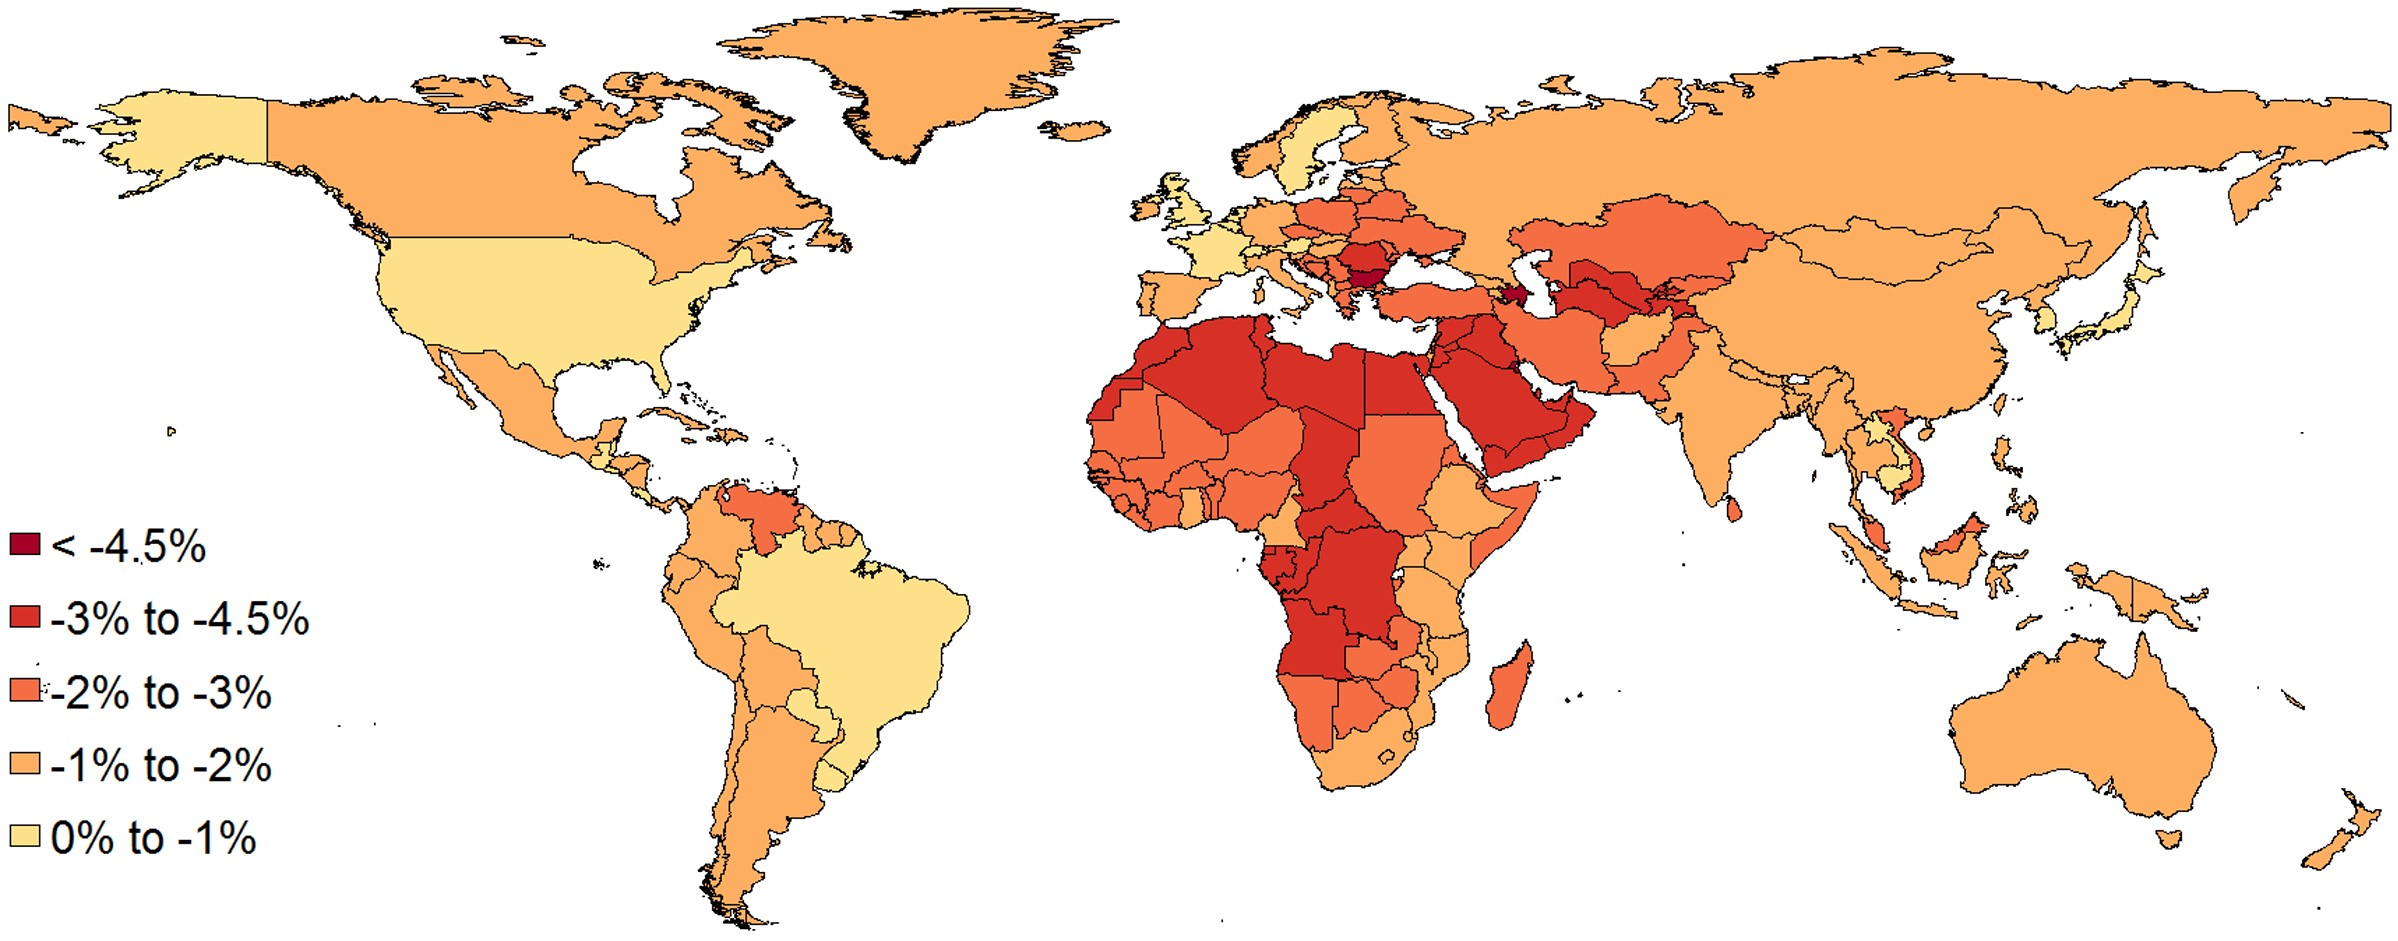
\includegraphics[width=0.48\textwidth]{img/A3-pure-tradeflows.jpg}
    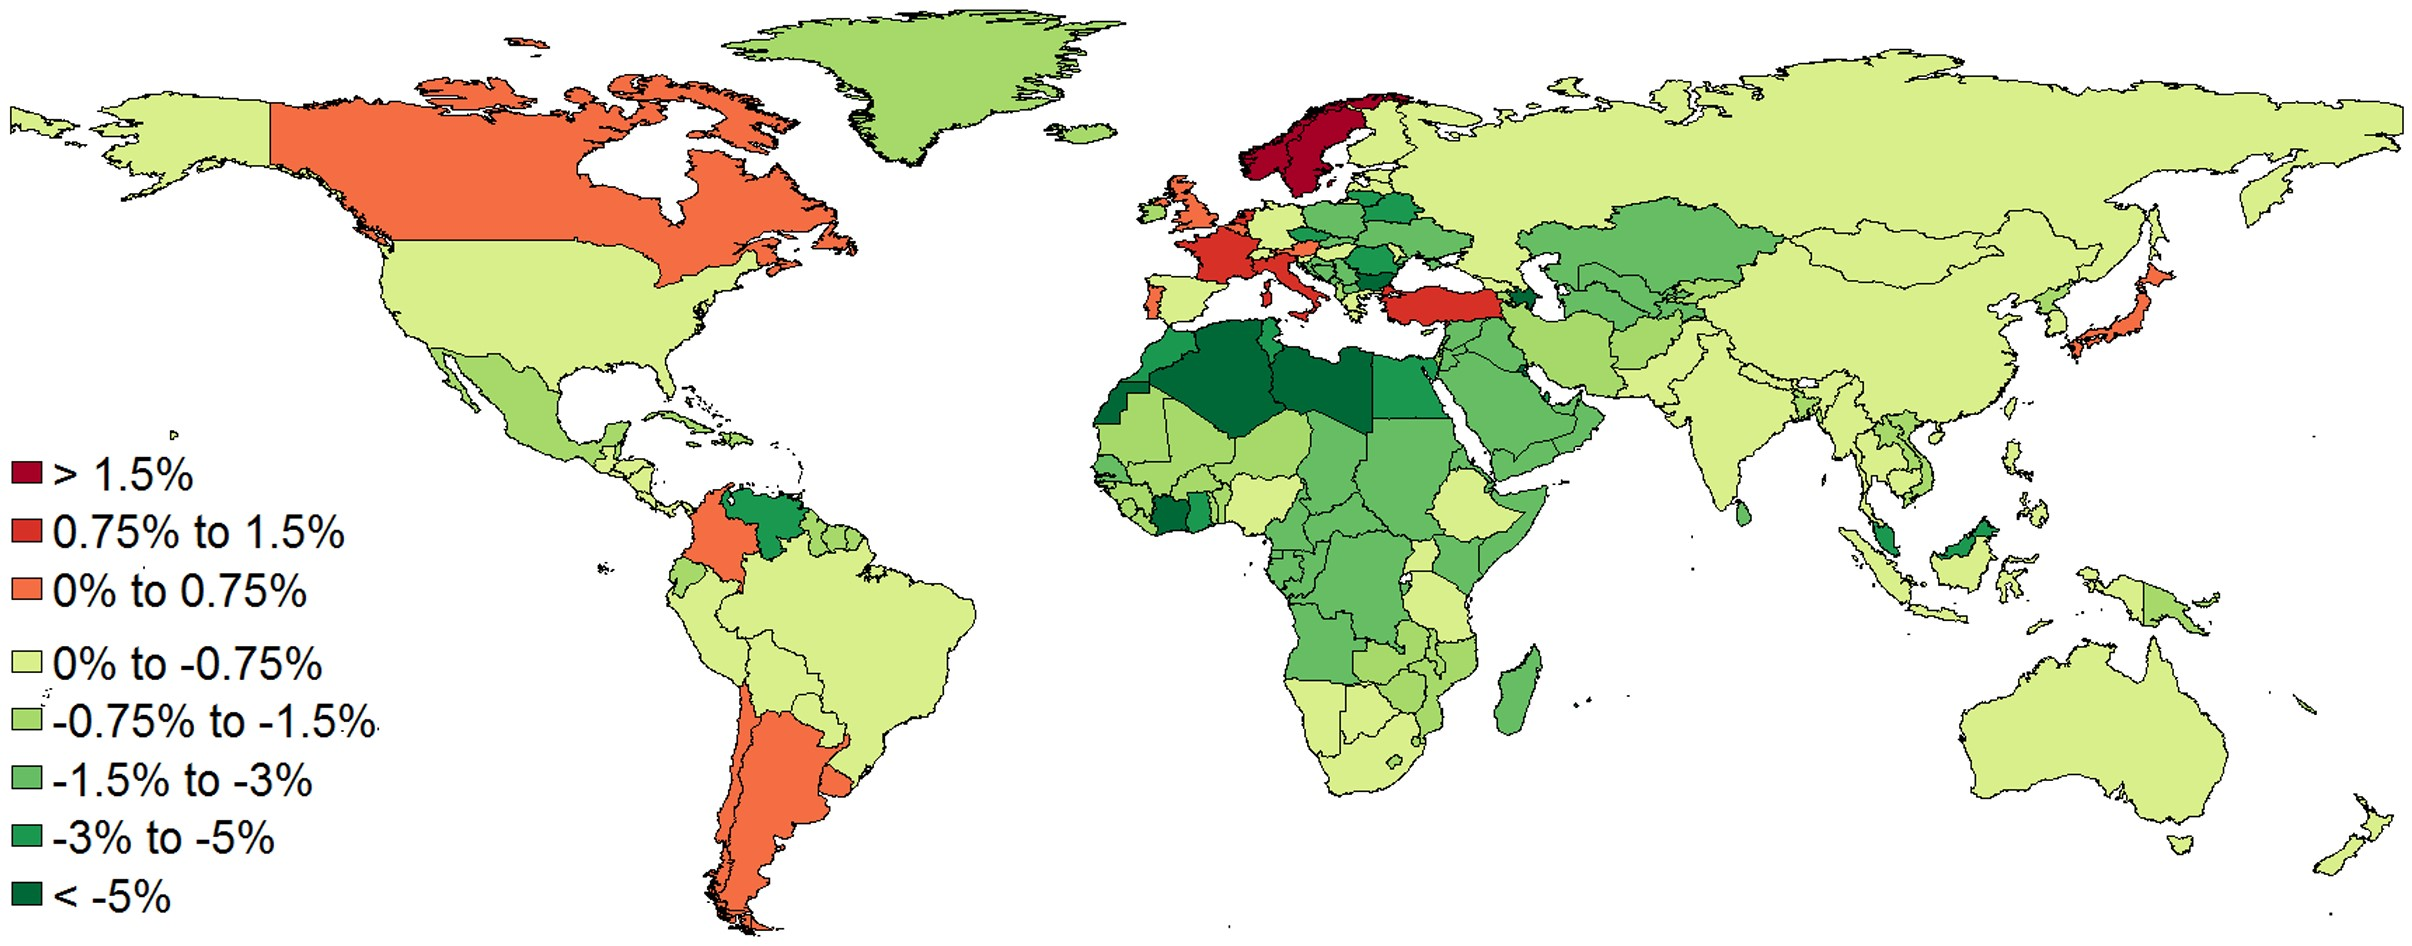
\includegraphics[width=0.48\textwidth]{img/A5-pure-emissions.jpg}
    \label{meta-analysis}
\end{figure}
\textbf{Trade flows -} The first result is that introducing pure carbon tariffs (i.e. equal to the country-pair differential in implicit carbon taxes $\lambda^i$) reduces global trade flows by $1.9\%$. In particular, countries with lower implicit carbon taxes suffer a stronger reduction in trade flows since (1) they will be asked the highest tariffs (their goods become more expensive and lose competitiveness), and (2) as can be seen in the gravity Equation \ref{eq:gravity}, tariffs negatively affects trade volumes.

\textbf{Welfare -} \textcite{Larch2017} measure welfare using the total utility function shown in Equation \ref{eq:CESutility} (b). Introducing pure carbon tariffs reduces welfare for the majority of countries, and most of them are developing countries in Africa and Asia. Utility falls as carbon tariffs increase the price $p_l^{ij}$ of tradable goods, negatively affect the budget constraint, and reduce the quantity $q_l^{ij}$ of goods consumed.

\textbf{Carbon emissions -} Lastly, carbon tariffs reduce global carbon emissions by $0.5\%$. As can be seen in Figure \ref{img:purecarbontariffs} on the right, they alter where emissions are produced. Previously, we mentioned that countries with low implicit carbon taxes see their trade flows decrease, since the production of those goods is shifted back to states with higher carbon taxes ("composition effect" between countries). By decomposing the effects on emissions, it can be seen that the decline in emissions is driven by a negative scale effect for all countries, which means that production in real terms declines everywhere. However, the composition effect appears to be the main driver of the reduction. In fact, it is negative for $80\%$ of the countries and accounts for $66\%$ of the global carbon emission contraction, meaning that most countries shift to less energy-intensive sectors, while the other share, consisting mainly of high carbon tax states, increases their emissions.

\subsection{Copenhagen Accord}

\textcite{Larch2017} also use their model to investigate the welfare and emissions impacts if a subset of countries, the Annex I group, were to meet the targets set in Appendix I of the Copenhagen Accord, signed in 2009 during the 15th session of the Conference of the Parties (COP). However, the partial adoption of emission targets and policies can lead to carbon leakage, therefore, the authors measure emissions that have not been cut, i.e. offset by non-committing countries, with the Leakage Rate (LR).

\textbf{Without tariffs -} Solving the counterfactual scenario given that Annex I countries fully commit to their emissions pledges results in a global carbon emission reduction of $8.4\%$. Responsible for $83.4\%$ of the global emissions reduction, the largest effect comes from the technique effect. In fact, exogenous emission commitments directly increase real energy prices, encouraging more efficient energy use. Leakage Rate reaches $13.4\%$.

\textbf{With tariffs -} Now, \textcite{Larch2017} include carbon tariffs to study their impact on the LR. Conversely from Section \ref{sec:purecarbontariffs}, they now amount to the real energy prices differential between committing and non-committing countries. With completely fulfilled targets by the committing countries and new carbon tariffs in place, the global carbon reduction is now stronger reaching $9.3\%$. This further increase is caused by a weaker composition effect (which typically increases emissions) and a stronger technique effect on average between the countries. Leakage Rate is reduced to $4.1\%$.